\pdfminorversion=4
\documentclass[aspectratio=169]{beamer}

\mode<presentation>
{
  \usetheme{default}
  \usecolortheme{default}
  \usefonttheme{default}
  \setbeamertemplate{navigation symbols}{}
  \setbeamertemplate{caption}[numbered]
  \setbeamertemplate{footline}[frame number]  % or "page number"
  \setbeamercolor{frametitle}{fg=white}
  \setbeamercolor{footline}{fg=black}
} 

\usepackage[english]{babel}
\usepackage[utf8x]{inputenc}
\usepackage{tikz}
\usepackage{courier}
\usepackage{array}
\usepackage{bold-extra}
\usepackage{minted}
\usepackage[thicklines]{cancel}
\usepackage{fancyvrb}

\xdefinecolor{dianablue}{rgb}{0.18,0.24,0.31}
\xdefinecolor{darkblue}{rgb}{0.1,0.1,0.7}
\xdefinecolor{darkgreen}{rgb}{0,0.5,0}
\xdefinecolor{darkgrey}{rgb}{0.35,0.35,0.35}
\xdefinecolor{darkorange}{rgb}{0.8,0.5,0}
\xdefinecolor{darkred}{rgb}{0.7,0,0}
\definecolor{darkgreen}{rgb}{0,0.6,0}
\definecolor{mauve}{rgb}{0.58,0,0.82}

\title[2018-09-18-jlab-reprise]{Data analysis tools from within particle physics and from industry}
\author{Jim Pivarski}
\institute{Princeton University -- DIANA-HEP}
\date{September 18, 2018}

\usetikzlibrary{shapes.callouts}

\begin{document}

\logo{\pgfputat{\pgfxy(0.11, 7.4)}{\pgfbox[right,base]{\tikz{\filldraw[fill=dianablue, draw=none] (0 cm, 0 cm) rectangle (50 cm, 1 cm);}\mbox{\hspace{-8 cm}
\includegraphics[height=1 cm]{princeton-logo-long.png}
\includegraphics[height=1 cm]{diana-hep-logo-long.png}}}}}

\begin{frame}
  \titlepage
\end{frame}

\logo{\pgfputat{\pgfxy(0.11, 7.4)}{\pgfbox[right,base]{\tikz{\filldraw[fill=dianablue, draw=none] (0 cm, 0 cm) rectangle (50 cm, 1 cm);}\mbox{\hspace{-8 cm}
\includegraphics[height=1 cm]{princeton-logo.png}
\includegraphics[height=1 cm]{diana-hep-logo.png}}}}}

% Uncomment these lines for an automatically generated outline.
%\begin{frame}{Outline}
%  \tableofcontents
%\end{frame}

% START START START START START START START START START START START START START

\begin{frame}{The point I want to make}
\large
\vspace{0.5 cm}
\begin{itemize}\setlength{\itemsep}{0.25 cm}
\item Although nuclear and high energy physics once dealt with the world's largest datasets, this is no longer true. ``Big Data'' or (better) ``Web Scale'' analysis regularly deals with petabytes and exabytes, and they've developed software tools for it.

\item<2-> We can reduce maintenance costs and improve students' career options by mixing industry standard tools with our in-house tools, particularly for cases in which the purpose of the tool is the same.

\item<3-> This is in line with ROOT's new Python and TMVA interfaces, but broader: data should flow freely to the best tool for the job and back again, leaving the choice in the physicist's hands.
\end{itemize}

\uncover<4->{\textcolor{darkblue}{In short, we should become like other sciences, such as astronomy or biology: common libraries for common stuff and our own libraries for domain-specific stuff.}}
\end{frame}

\begin{frame}{\only<1>{We measure globally distributed data in hundreds of PB}\only<2>{But for web scale companies, 100 PB = 1 truck}}
\vspace{0.35 cm}
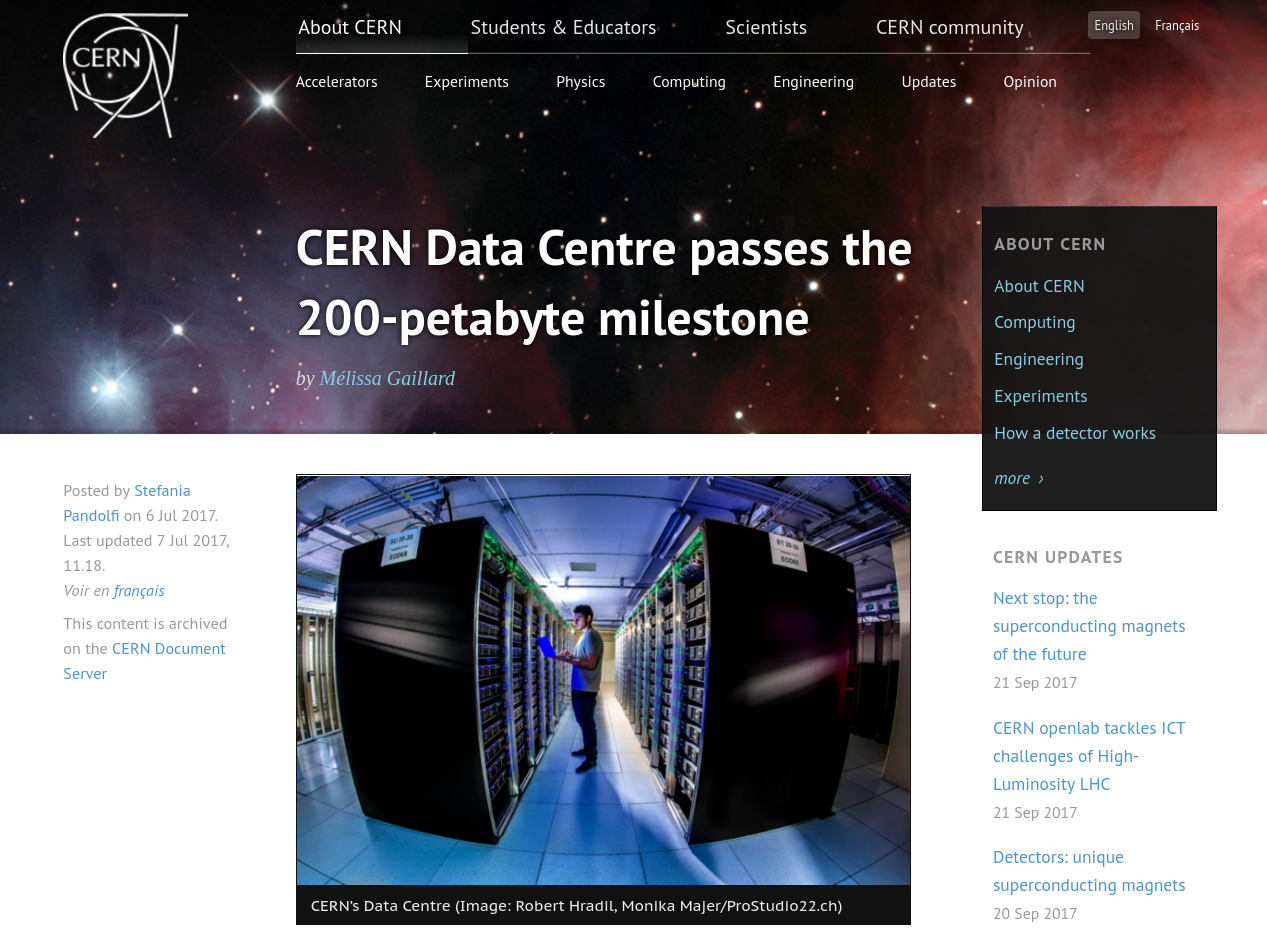
\includegraphics[width=0.73\linewidth]{cern-200pb.png}

\vspace{-4.8 cm}
\uncover<2->{\mbox{ } \hfill 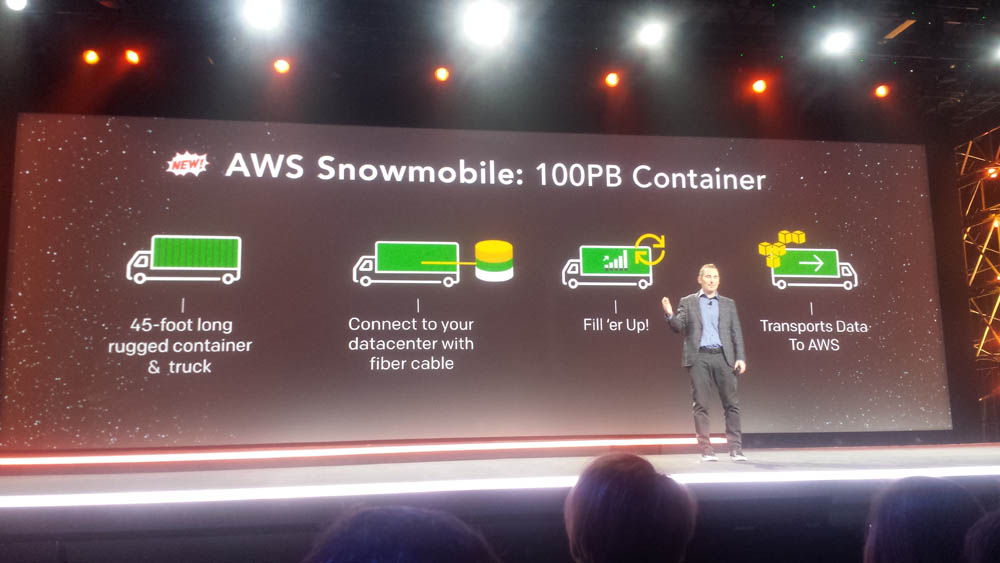
\includegraphics[width=0.7\linewidth]{aws-snowmobile.jpg}\hspace{-1 cm}}
\end{frame}

\begin{frame}{Number of people (users and developers) also dwarf our field}
\vspace{0.25 cm}
\mbox{ } \hfill 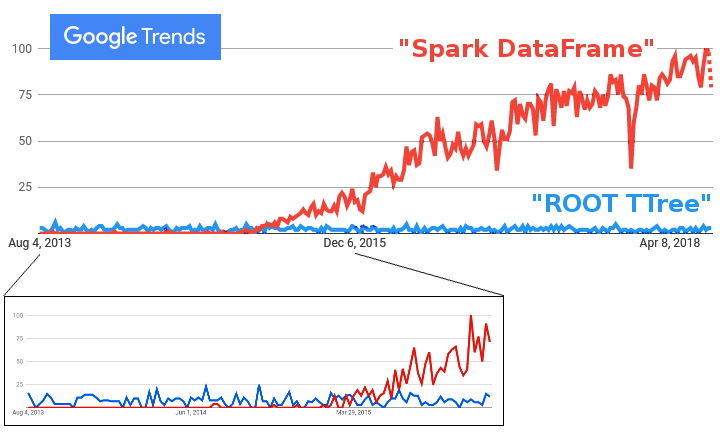
\includegraphics[width=0.9\linewidth]{root-spark-google-trends.png} \hfill \mbox{ }
\end{frame}

\begin{frame}{Number of people (users and developers) also dwarf our field}
\large
\vspace{0.5 cm}
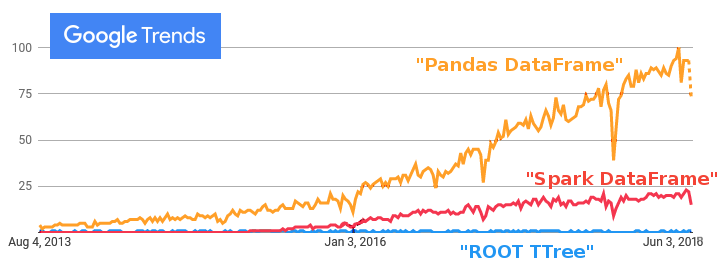
\includegraphics[width=\linewidth]{root-spark-pandas-google-trends.png}

\vspace{0.5 cm}
\uncover<2->{More users means more bug reports, more online help, more how-to blogs\ldots}

\vspace{0.2 cm}
\uncover<2->{More developers means more bug-fixes, more features, more connectors\ldots}
\end{frame}

\begin{frame}{Another important metric: experience!}
\Large
\vspace{0.25 cm}
\begin{itemize}\setlength{\itemsep}{0.25 cm}
\item Physicists have been performing big data analytics (reducing large datasets to statistical inferences) for about \textcolor{darkblue}{\underline{50 years}}.

\item Web scale companies have been doing it for about \textcolor{darkblue}{\underline{10 years}}.
\end{itemize}

\vspace{0.5 cm}
\uncover<2->{Nuclear and high-energy physics analysis is specialized and sophisticated--- many tools we'd call ``basic'' are not implemented in industry-grade software.}

\vspace{0.5 cm}
\uncover<3->{The simple prescription of ``just use Spark'' would leave analyzers without some necessary tools.}
\end{frame}

\begin{frame}{What should we do?}
\large
\vspace{0.5 cm}
\begin{columns}[t]
\column{0.25\linewidth}
\textcolor{darkblue}{\underline{Option \#1}}

\vspace{0.25 cm}
All of our needs are specialized.

\vspace{0.25 cm}
Continue developing our own everything.

\vspace{2.5 cm}

\column{0.25\linewidth}
\begin{uncoverenv}<2->
\textcolor{darkblue}{\hspace{-0.18 cm}\underline{Option \#2}}

\vspace{0.25 cm}
Modern big data software has some good ideas; integrate those \underline{\it ideas} into our stack.
\end{uncoverenv}

\column{0.25\linewidth}
\begin{uncoverenv}<3->
\only<3-4>{\textcolor{darkblue}{\hspace{-0.18 cm}\underline{Option \#3}}}\only<5->{\textcolor{darkorange}{\hspace{-0.18 cm}\underline{Option \#3}}}

\vspace{0.25 cm}
\only<3-4>{Narrow our scope to domain-specific tools, what no one else is developing, and make them interoperate with non-physics tools for the common parts.}\only<5->{\textcolor{darkorange}{Narrow our scope to domain-specific tools, what no one else is developing, and make them interoperate with non-physics tools for the common parts.}}
\end{uncoverenv}

\column{0.25\linewidth}
\begin{uncoverenv}<4->
\textcolor{darkblue}{\hspace{-0.18 cm}\underline{Option \#4}}

\vspace{0.25 cm}
Convince the world to start using physics analysis techniques so that they will develop solutions for these, too.
\end{uncoverenv}
\end{columns}

\vspace{0.5 cm}
\uncover<5->{\textcolor{darkorange}{\bf \#3 is my opinion, but what's domain-specific and what's not?}}
\end{frame}

\begin{frame}{Three examples each:}
\Large
\vspace{-0.5 cm}
\begin{columns}[t]
\column{0.5\linewidth}
\mbox{\hspace{0.25 cm}\textcolor{darkblue}{\underline{What web scale software's got}}}

\vspace{0.25 cm}
\begin{enumerate}
\item Distributed DAG processing
\item Indexed analysis
\item Machine learning
\end{enumerate}

\column{0.5\linewidth}
\mbox{\hspace{0.45 cm}\textcolor{darkblue}{\underline{What we need that it hasn't got}}}

\vspace{0.25 cm}
\begin{enumerate}
\item Nested data structures
\item Advanced histogramming
\item Ansatz fitting
\end{enumerate}

\end{columns}
\end{frame}

\begin{frame}{}
\huge
\vspace{0.5 cm}
\begin{center}
\textcolor{darkblue}{Distributed DAG processing}

\large
\vspace{0.5 cm}
not physics-specific
\end{center}
\end{frame}

\begin{frame}{Distributed DAG processing}
\large
\vspace{0.5 cm}
\begin{columns}
\column{0.21\linewidth}
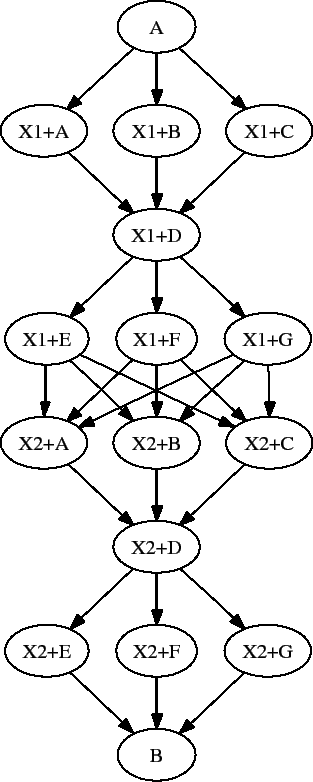
\includegraphics[width=\linewidth]{dag-htcondor.png}

\column{0.83\linewidth}
DAG: Directed Acyclic Graph of dependencies between subtasks.

Some would say this is what big data processing \underline{\it is}.

\vspace{1 cm}
Many frameworks distribute work this way:

\vspace{0.2 cm}
\hfill \begin{minipage}{0.95\linewidth}
\textcolor{darkblue}{Spark} (JVM), \textcolor{darkblue}{Dask}, \textcolor{darkblue}{Joblib}, \textcolor{darkblue}{Parsl} (Python), \textcolor{darkblue}{Storm} (continuous), \textcolor{darkblue}{Thrill} (C++), \textcolor{darkblue}{DAGMan} (HTCondor), \textcolor{darkblue}{TensorFlow} (fitting)\ldots
\end{minipage}

\vspace{1 cm}
Physics software is embracing this approach:

\begin{itemize}
\item RDataFrame in ROOT
\item Dozens of other examples at CHEP
\end{itemize}
\end{columns}
\end{frame}

\begin{frame}{RDataFrame from the ROOT Workshop (last week)}
\vspace{0.25 cm}
\only<1>{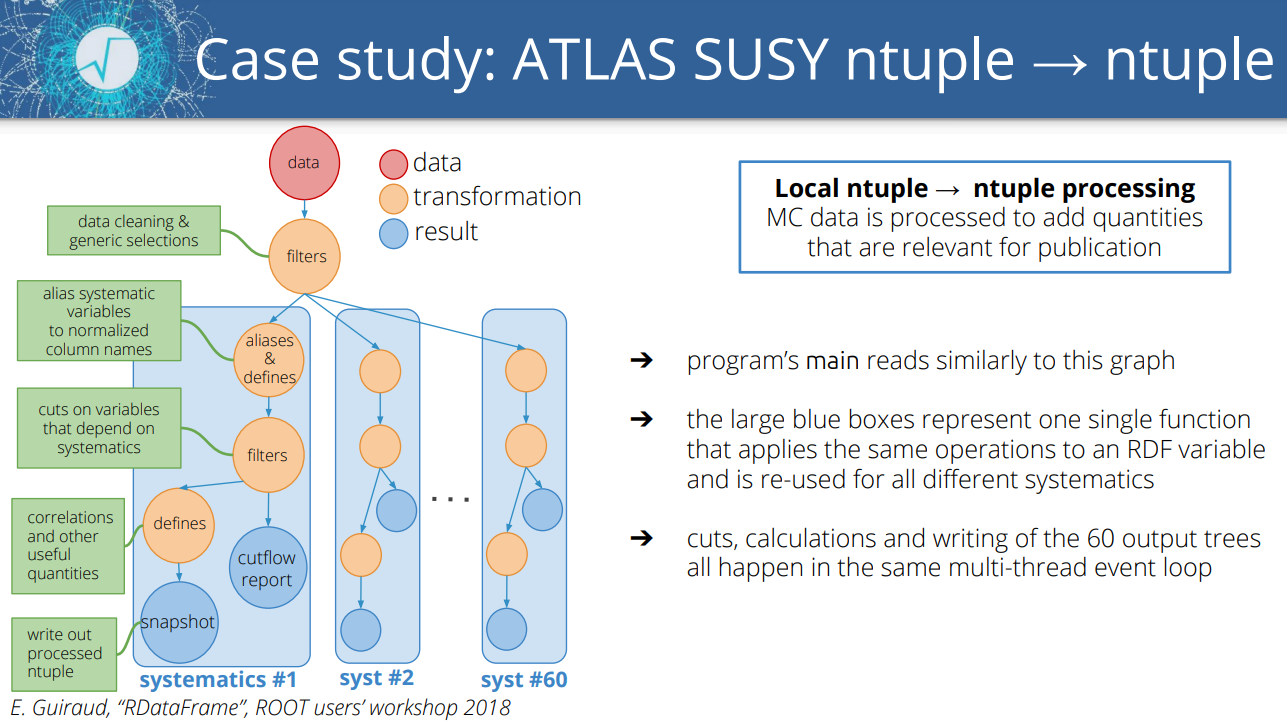
\includegraphics[width=\linewidth]{rdataframe-use-case-1.png}}
\only<2>{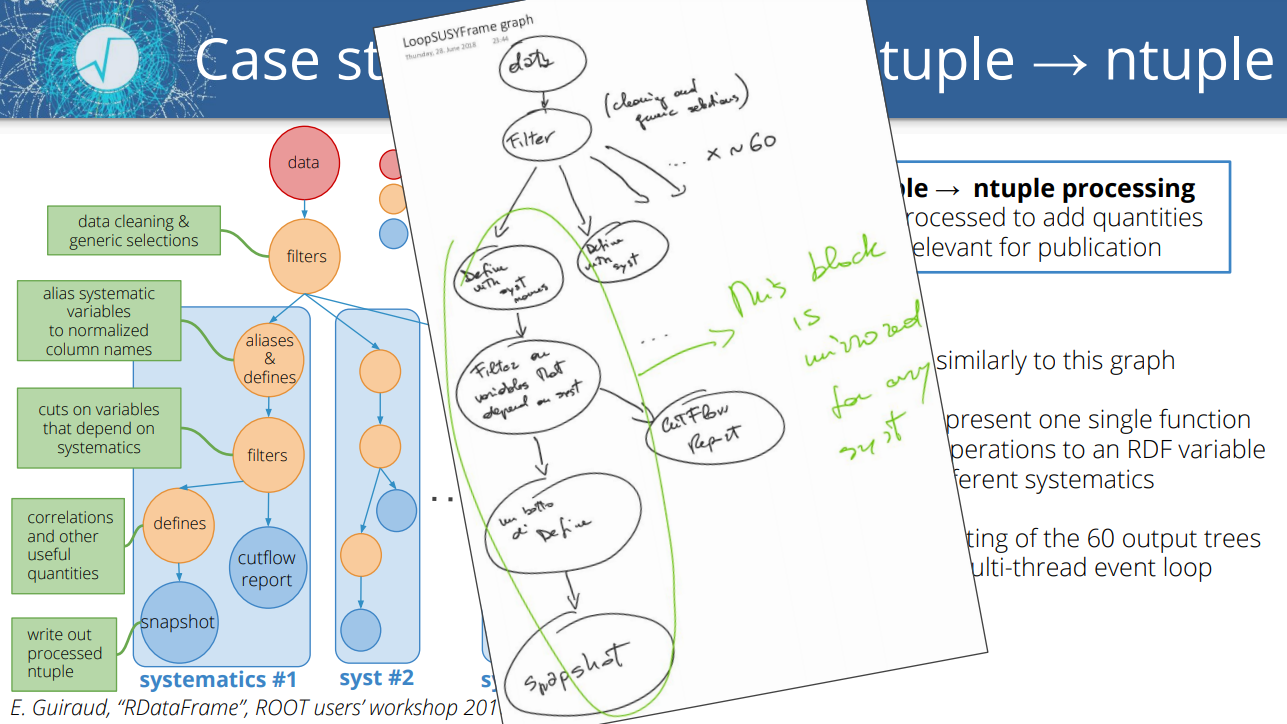
\includegraphics[width=\linewidth]{rdataframe-use-case-2.png}}
\end{frame}

\begin{frame}{But how will it develop?}
\Large
\vspace{0.5 cm}
\begin{columns}
\column{0.9\linewidth}
Will RDataFrame be a {\it programming model} that {\it interfaces} with distributed processing systems such as Spark?

\vspace{0.5 cm}
Or will it be {\it part} of a ROOT {\it implementation} of distributed DAG processing? A new PROOF, for instance?
\end{columns}

\vspace{1 cm}
\uncover<2->{\textcolor{darkblue}{Distributing computational tasks with dependencies is a good example of a non-domain-specific problem.}}
\end{frame}

\begin{frame}{}
\huge
\vspace{0.5 cm}
\begin{center}
\textcolor{darkblue}{Nested data structures}

\large
\vspace{0.5 cm}
strangely physics-specific, but shouldn't be
\end{center}
\end{frame}

\begin{frame}{Nested data structures}
\large
\vspace{0.5 cm}
\begin{columns}[t]
\column{0.5\linewidth}
\mbox{ } \hfill 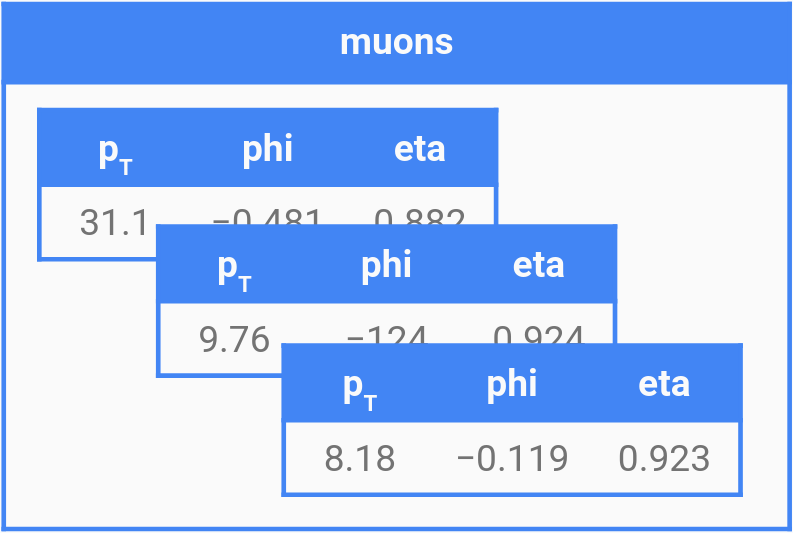
\includegraphics[width=0.75\linewidth]{muons-as-objects.png} \hfill \mbox{ }

\vspace{0.25 cm}
\begin{uncoverenv}<2->
Objects are essential in physics analysis.

\vspace{0.25 cm}
Many physicists consider TTrees with {\tt\small std::vector<float>} branches to be ``minimal'' or ``flat.''
\end{uncoverenv}

\column{0.5\linewidth}
\mbox{ } \hfill 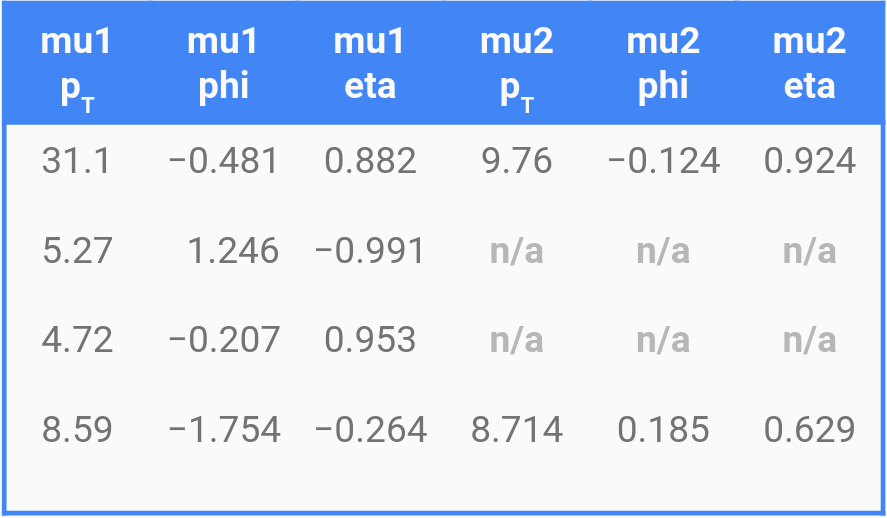
\includegraphics[width=0.75\linewidth]{muons-as-a-table.png} \hfill \mbox{ }

\vspace{0.25 cm}
\begin{uncoverenv}<3->
Most data analysis tools have an SQL mindset, with rectangular data tables.

\vspace{0.25 cm}
\textcolor{darkblue}{Objects $\to$ rectangular tables is lossy!}

\vspace{0.25 cm}
Performance claims often start the stopwatch after this ``data cleaning.''
\end{uncoverenv}
\end{columns}
\end{frame}

\begin{frame}{Nested data structures}
\large
\vspace{0.5 cm}
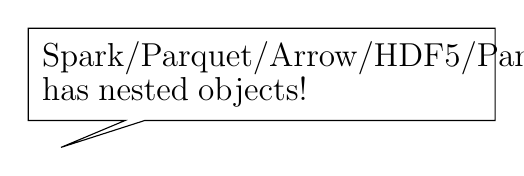
\begin{tikzpicture}[>=latex]
\node[rectangle callout, draw, inner sep=5 pt, callout relative pointer={(200:1 cm)}, text width=0.46\linewidth] {\large Spark/Parquet/Arrow/HDF5/Pandas has nested objects!};
\end{tikzpicture} \hfill \uncover<2->{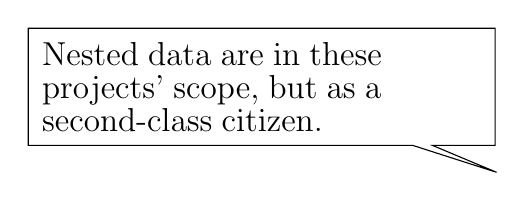
\begin{tikzpicture}[>=latex]
\node[rectangle callout, draw, inner sep=5 pt, callout relative pointer={(-200:-1 cm)}, text width=0.46\linewidth] {\large Nested data are in these projects' scope, but as a second-class citizen.};
\end{tikzpicture}}

\vspace{0.75 cm}
\begin{itemize}\setlength{\itemsep}{0.35 cm}
\item<3-> \textcolor{darkblue}{Spark} DataFrames allow arrays of structs, but using them involves a cumbersome explode-groupby or ``drop to RDDs,'' giving up performance.
\item<4-> \textcolor{darkblue}{Parquet} and \textcolor{darkblue}{Arrow} specifications define lists of records, but they haven't been implemented in C++ and therefore Python yet (last time I checked).
\item<5-> \textcolor{darkblue}{HDF5} has lists of compounds, but they're rowwise (``unsplit'').
\item<6-> \textcolor{darkblue}{Pandas} can put arbitrary Python objects in DataFrames, but most operations only apply to numbers.
\end{itemize}
\end{frame}

\begin{frame}[fragile]{Nested data structures}
\tiny
\vspace{0.25 cm}
\hfill 
\includegraphics[height=1 cm]{uproot-logo.pdf}

\vspace{-1.1 cm}
\begin{onlyenv}<1>\begin{minted}{python}
>>> import uproot
>>> t = uproot.open("tests/samples/HZZ.root")["events"]
>>> t.pandas.df(["MET_px", "Muon_Px", "Electron_Px"], entrystart=-20, flatten=False)
\end{minted}
\end{onlyenv}\begin{onlyenv}<2>\begin{minted}{python}
>>> import uproot
>>> t = uproot.open("tests/samples/HZZ.root")["events"]
>>> t.pandas.df(["MET_px", "Muon_Px", "Electron_Px"], entrystart=-20, flatten=True)
\end{minted}
\end{onlyenv}
\begin{onlyenv}<1>\begin{verbatim}
         MET_px                  Muon_Px              Electron_Px
2401   2.998099              [-1.492689]                       []
2402  27.944883              [-4.560287]                       []
2403   3.787466              [-9.715589]                       []
2404   9.378232             [-31.072098]                       []
2405 -17.310106   [47.484627, 4.6953125]                       []
2406 -81.965927   [74.75617, -20.911081]                       []
2407  -9.059591  [25.786427, -29.265024]                       []
2408  25.649775                       []                       []
2409  29.691553               [-24.7368]                       []
2410 -25.754967  [53.005814, -30.208649]  [-37.681973, 18.453588]
2411  -2.426847    [55.7203, -26.914448]                       []
2412 -15.611773              [14.896802]                       []
2413  18.921183             [-24.158083]                       []
2414 -11.730723              [-9.204197]                       []
2415 -10.648725   [34.506527, -31.56778]                       []
2416 -14.607650             [-39.285824]                       []
2417  22.208313              [35.067146]                       []
2418  18.101646             [-29.756786]                       []
2419  79.875191              [1.1418698]                       []
2420  19.713749              [23.913206]                       []
\end{verbatim}
\vspace{1.7 cm}
\end{onlyenv}\begin{onlyenv}<2>\begin{verbatim}
                   MET_px     Muon_Px  Electron_Px
entry subentry
2401  0          2.998099  -1.492689          NaN
2402  0         27.944883  -4.560287          NaN
2403  0          3.787466  -9.715589          NaN
2404  0          9.378232 -31.072098          NaN
2405  0        -17.310106  47.484627          NaN
      1               NaN   4.695312          NaN
2406  0        -81.965927  74.756172          NaN
      1               NaN -20.911081          NaN
2407  0         -9.059591  25.786427          NaN
      1               NaN -29.265024          NaN
2408  0         25.649775        NaN          NaN
2409  0         29.691553 -24.736799          NaN
2410  0        -25.754967  53.005814   -37.681973
      1               NaN -30.208649    18.453588
2411  0         -2.426847  55.720299          NaN
      1               NaN -26.914448          NaN
2412  0        -15.611773  14.896802          NaN
2413  0         18.921183 -24.158083          NaN
2414  0        -11.730723  -9.204197          NaN
2415  0        -10.648725  34.506527          NaN
      1               NaN -31.567780          NaN
2416  0        -14.607650 -39.285824          NaN
2417  0         22.208313  35.067146          NaN
2418  0         18.101646 -29.756786          NaN
2419  0         79.875191   1.141870          NaN
2420  0         19.713749  23.913206          NaN
\end{verbatim}
\end{onlyenv}

\vspace{-5 cm}
\hfill \begin{minipage}{0.33\linewidth}
\large
\textcolor{darkblue}{In some cases, maybe we're using the wrong idiom:} instead of working with structured values, Pandas prefers structured indexes.
\end{minipage}
\vspace{5 cm}
\end{frame}

\begin{frame}[fragile]{Nested data structures}
\large
\vspace{0.4 cm}
But that shouldn't be the only way: we {\it should} be able to use our data models and algorithms, even if we run them in non-physics frameworks.

\begin{uncoverenv}<2->
\vspace{0.5 cm}
This is my main project now: \textcolor{darkblue}{fast manipulation of columnar data.}

\vspace{0.25 cm}
\hfill 
\includegraphics[height=1 cm]{awkward-logo.pdf}

\vspace{0.25 cm}
\vspace{-1 cm}
\scriptsize
\begin{columns}[t]
\column{0.405\linewidth}
\underline{\large General programming model}

\begin{minted}{python}
@numba.jit    # LLVM-compiled Python
def deltaphi(event):
    metphi = event.MET.phi
    for jet in event.jets:
        yield metphi - jet.phi
\end{minted}

\column{0.525\linewidth}
\underline{\large Numpy-like broadcasting}

\vspace{\baselineskip}
\begin{minted}{python}
# one per event       one per particle
event["MET"]["phi"] - event["jet"]["phi"]
\end{minted}
\end{columns}
\end{uncoverenv}

\large
\vspace{0.7 cm}
\uncover<3->{Also, this {\it should} be of wider interest than physics: developers of Arrow, Dask, and XND ($\sim$Numpy 2.0) are curious about it.}
\end{frame}

\begin{frame}{Missed opportunity}
\begin{center}
\only<1>{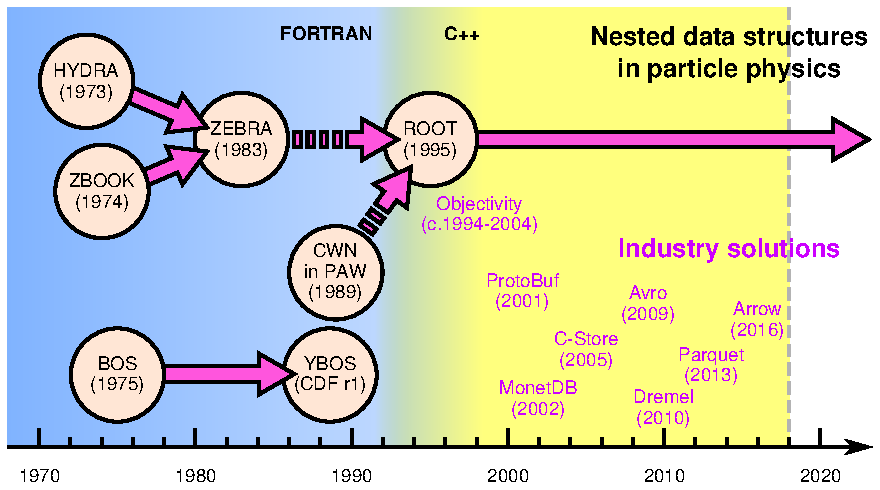
\includegraphics[width=\linewidth]{history.pdf}}\only<2->{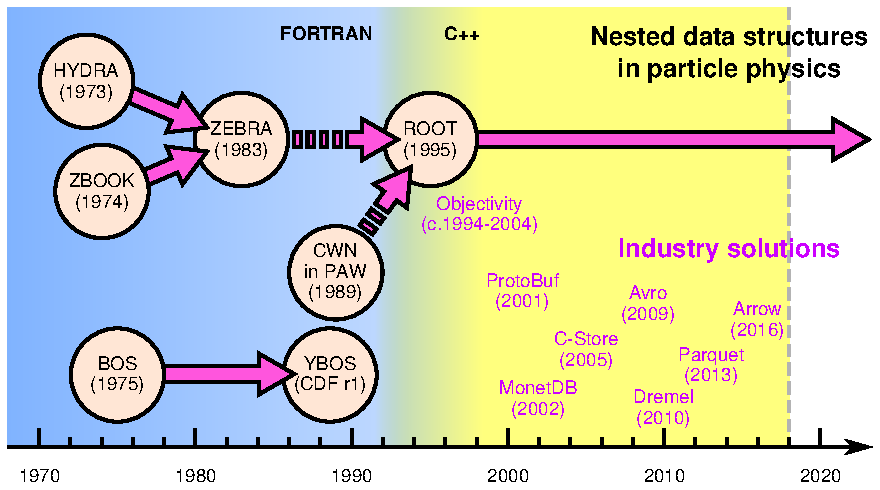
\includegraphics[width=0.7\linewidth]{history.pdf}}
\end{center}
\begin{uncoverenv}<2->
\begin{columns}
\column{0.43\linewidth}
\begin{center}
\small
{\Large Google Dremel paper (2010):}

\textcolor{gray}{(inspired Parquet)}
\end{center}

\column{0.65\linewidth}
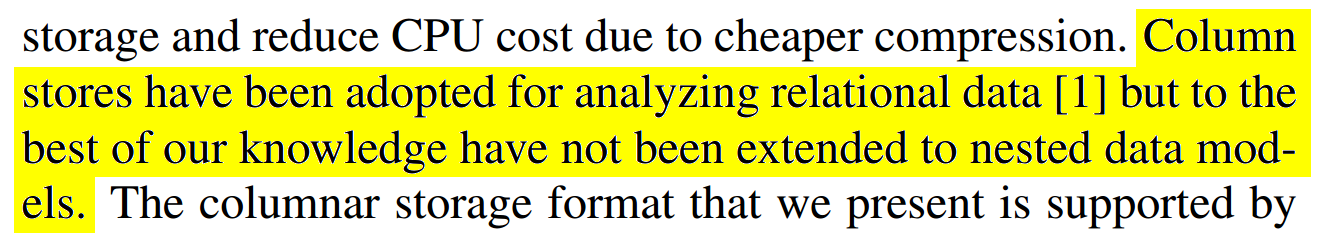
\includegraphics[width=\linewidth]{dremel-paper-cropped.png}
\end{columns}
\end{uncoverenv}
\end{frame}

\begin{frame}{}
\huge
\vspace{0.5 cm}
\begin{center}
\textcolor{darkblue}{Indexed analysis}

\large
\vspace{0.5 cm}
not well-known in our field
\end{center}
\end{frame}

\begin{frame}{What is indexing?}
\large
\vspace{0.5 cm}
\textcolor{darkblue}{\Large A way of organizing analysis:}

\vspace{0.25 cm}
\begin{itemize}\setlength{\itemsep}{0.25 cm}
\item PAW/HBOOK histograms were indexed by \underline{\it integer IDs}
\item ROOT histograms are indexed by \underline{\it string names}
\item ROOT TTrees are indexed by \underline{\it integer entry numbers}
\item Excel spreadsheets are indexed by \underline{\it integer row and letter column IDs}
\item SQL tables are indexed by \underline{\it unordered sets}
\item Pandas DataFrames are indexed by \underline{\it ordered, structured series}
\end{itemize}
\end{frame}

\begin{frame}[fragile]{Pandas is not a TTree replacement!}
\large
\vspace{0.5 cm}
Most of Pandas's functionality is about manipulating data by index, and the whole DataFrame must fit in memory.

\small
\begin{minted}{python}
result = left.join(right, how="inner")
\end{minted}
\large

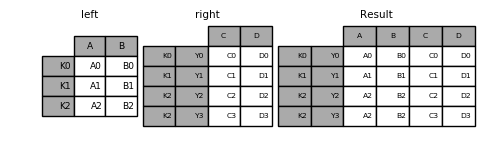
\includegraphics[width=0.7\linewidth]{merging_join_multiindex_inner.png}

\vspace{0.5 cm}
None (?) of TTree's functionality is about manipulating data by index, and it's focused on lazily loading large datasets.
\end{frame}

\begin{frame}[fragile]{Pandas DataFrames resemble histograms, not TTrees}
\large
\vspace{0.5 cm}
Histograms are mappings from intervals to weighted counts and their errors.

\vspace{0.5 cm}
Profiles are mappings from intervals to weighted means and standard deviations.

\vspace{0.5 cm}
Pandas has an interval key type, as well as MultiIndexes for multiple dimensions.

\vspace{0.5 cm}
Since the index is explicit, rather than by position in an array, there's no distinction between sparse and dense histograms. (Drop zero-valued rows and impute zero on merge.)

\vspace{0.5 cm}
Fluidly convert between MultiIndexes and columns with {\normalsize\mintinline{python}{pivot_table()}}.

\vspace{0.5 cm}
\textcolor{gray}{(Stop making arrays and {\normalsize\mintinline{python}{std::maps}} of TH3!)}
\end{frame}

\begin{frame}[fragile]{Indexed analysis}
\large
\vspace{0.25 cm}
\hfill 
\includegraphics[height=1 cm]{histbook-logo.pdf}

\vspace{-1 cm}
\scriptsize
\begin{onlyenv}<1>
\scriptsize
\begin{minted}{python}
>>> from histbook import *
>>> multihist = Hist(
...     bin("mass", 100, 0, 500), cut("q1*q2 < 0"),
...     split("mt1", [0.2, 0.5]), split("mt2", [0.2, 0.5]), fill=df)
>>> multihist.pandas()
\end{minted}
\scriptsize
\vspace{-0.25 cm}
\begin{verbatim}
                   MultiIndex key                         Columns
--------------------------------------------------+---------------------
                                                  | count() err(count())
mass           q1*q2 < 0 mt1         mt2          |
[-inf, 0.0)    fail      [-inf, 0.2) [-inf, 0.2)  |     0.0          0.0
                                     [0.2, 0.5)   |     0.0          0.0
                                     [0.5, inf)   |     0.0          0.0
                         [0.2, 0.5)  [-inf, 0.2)  |     0.0          0.0
                                     [0.2, 0.5)   |     0.0          0.0
                                     [0.5, inf)   |     0.0          0.0
                         [0.5, inf)  [-inf, 0.2)  |     0.0          0.0
                                     [0.2, 0.5)   |     0.0          0.0
                                     [0.5, inf)   |     0.0          0.0
               pass      [-inf, 0.2) [-inf, 0.2)  |     0.0          0.0
                                     [0.2, 0.5)   |     0.0          0.0
                                     [0.5, inf)   |     0.0          0.0
                         [0.2, 0.5)  [-inf, 0.2)  |     0.0          0.0
                                     [0.2, 0.5)   |     0.0          0.0
                                     [0.5, inf)   |     0.0          0.0
                         [0.5, inf)  [-inf, 0.2)  |     0.0          0.0
                                     [0.2, 0.5)   |     0.0          0.0
\end{verbatim}
\end{onlyenv}
\begin{onlyenv}<2>
\scriptsize
\begin{minted}{python}
>>> from histbook import *
>>> multihist = Hist(
...     bin("mass", 100, 0, 500), cut("q1*q2 < 0"),
...     split("mt1", [0.2, 0.5]), split("mt2", [0.2, 0.5]), fill=df)
>>> multihist.step("mass")
\end{minted}
\mbox{ } \hfill 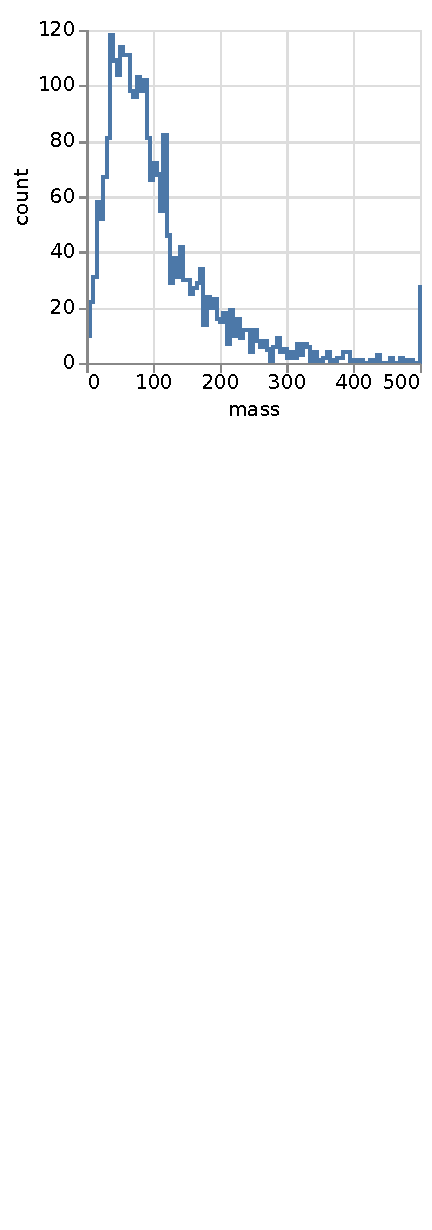
\includegraphics[height=6 cm]{pandhist.pdf} \hfill \mbox{ }
\end{onlyenv}
\begin{onlyenv}<3>
\scriptsize
\begin{minted}{python}
>>> from histbook import *
>>> multihist = Hist(
...     bin("mass", 100, 0, 500), cut("q1*q2 < 0"),
...     split("mt1", [0.2, 0.5]), split("mt2", [0.2, 0.5]), fill=df)
>>> multihist.overlay("q1*q2 < 0").step("mass")
\end{minted}
\mbox{ } \hfill 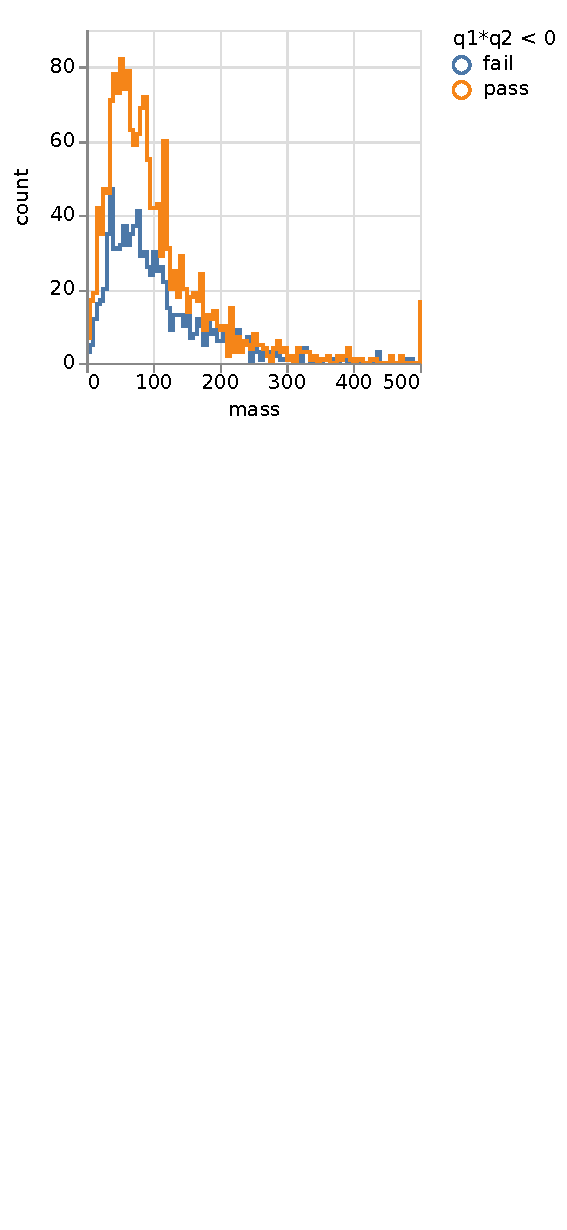
\includegraphics[height=6 cm]{pandhist_overlay.pdf} \hfill \mbox{ }
\end{onlyenv}
\begin{onlyenv}<4>
\scriptsize
\begin{minted}{python}
>>> from histbook import *
>>> multihist = Hist(
...     bin("mass", 100, 0, 500), cut("q1*q2 < 0"),
...     split("mt1", [0.2, 0.5]), split("mt2", [0.2, 0.5]), fill=df)
>>> multihist.stack("q1*q2 < 0").area("mass")
\end{minted}
\mbox{ } \hfill 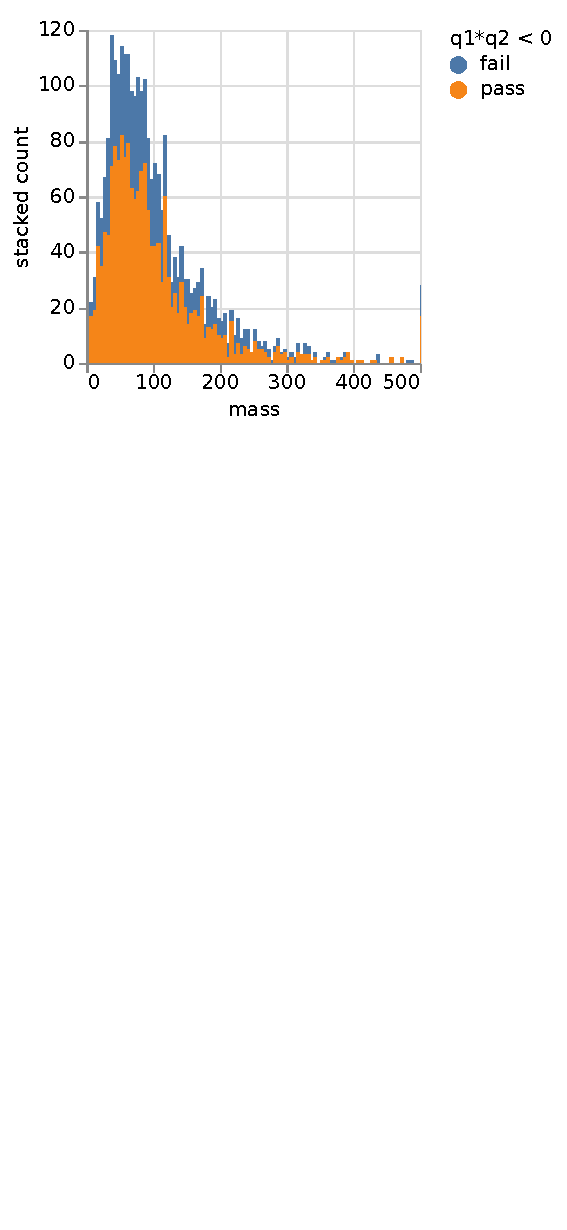
\includegraphics[height=6 cm]{pandhist_stack.pdf} \hfill \mbox{ }
\end{onlyenv}
\begin{onlyenv}<5>
\scriptsize
\begin{minted}{python}
>>> from histbook import *
>>> multihist = Hist(
...     bin("mass", 100, 0, 500), cut("q1*q2 < 0"),
...     split("mt1", [0.2, 0.5]), split("mt2", [0.2, 0.5]), fill=df)
>>> multihist.beside("q1*q2 < 0").step("mass")
\end{minted}
\mbox{ } \hfill 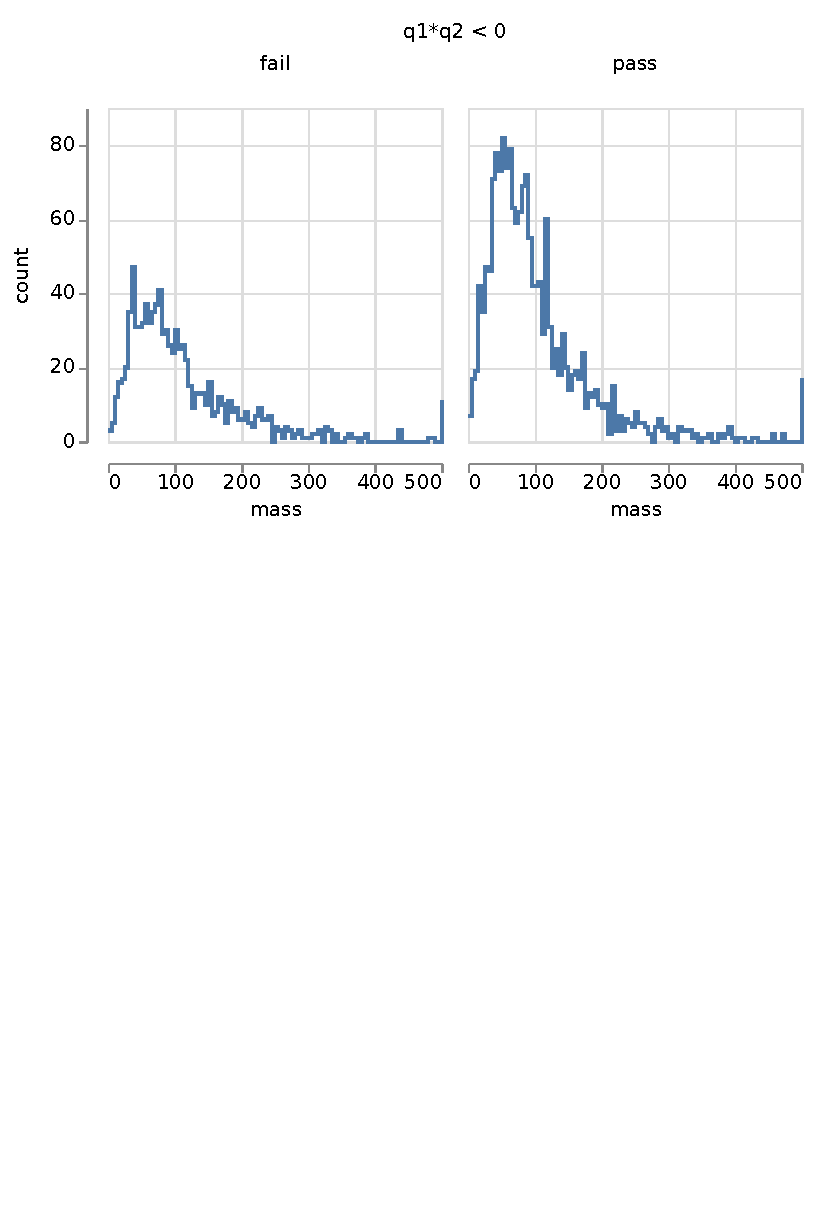
\includegraphics[height=6 cm]{pandhist_trellis.pdf} \hfill \mbox{ }
\end{onlyenv}
\begin{onlyenv}<6>
\scriptsize
\begin{minted}{python}
>>> from histbook import *
>>> multihist = Hist(
...     bin("mass", 100, 0, 500), cut("q1*q2 < 0"),
...     split("mt1", [0.2, 0.5]), split("mt2", [0.2, 0.5]), fill=df)
>>> multihist.below("mt1").beside("mt2").step("mass")
\end{minted}
\mbox{ } \hfill 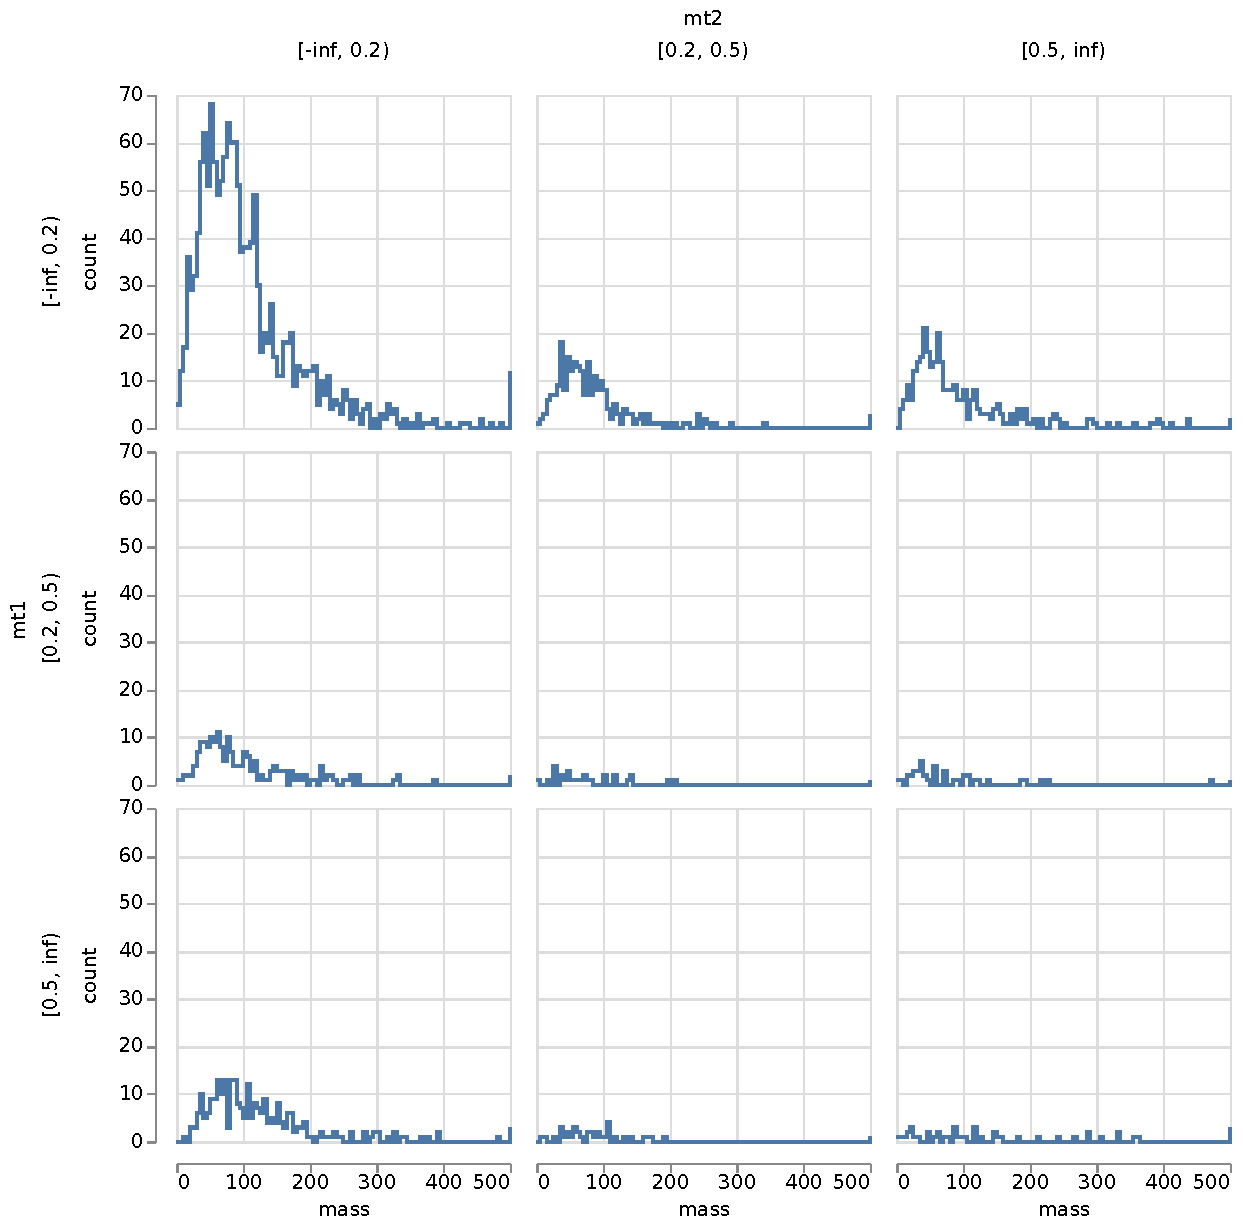
\includegraphics[height=6 cm]{pandhist_double_trellis.pdf} \hfill \mbox{ }
\end{onlyenv}
\begin{onlyenv}<7>
\scriptsize
\begin{minted}{python}
>>> from histbook import *
>>> multihist = Hist(
...     bin("mass", 100, 0, 500), cut("q1*q2 < 0"),
...     split("mt1", [0.2, 0.5]), split("mt2", [0.2, 0.5]), fill=df)
>>> multihist.below("mt1").beside("mt2").overlay("q1*q2 < 0").step("mass")
\end{minted}
\mbox{ } \hfill 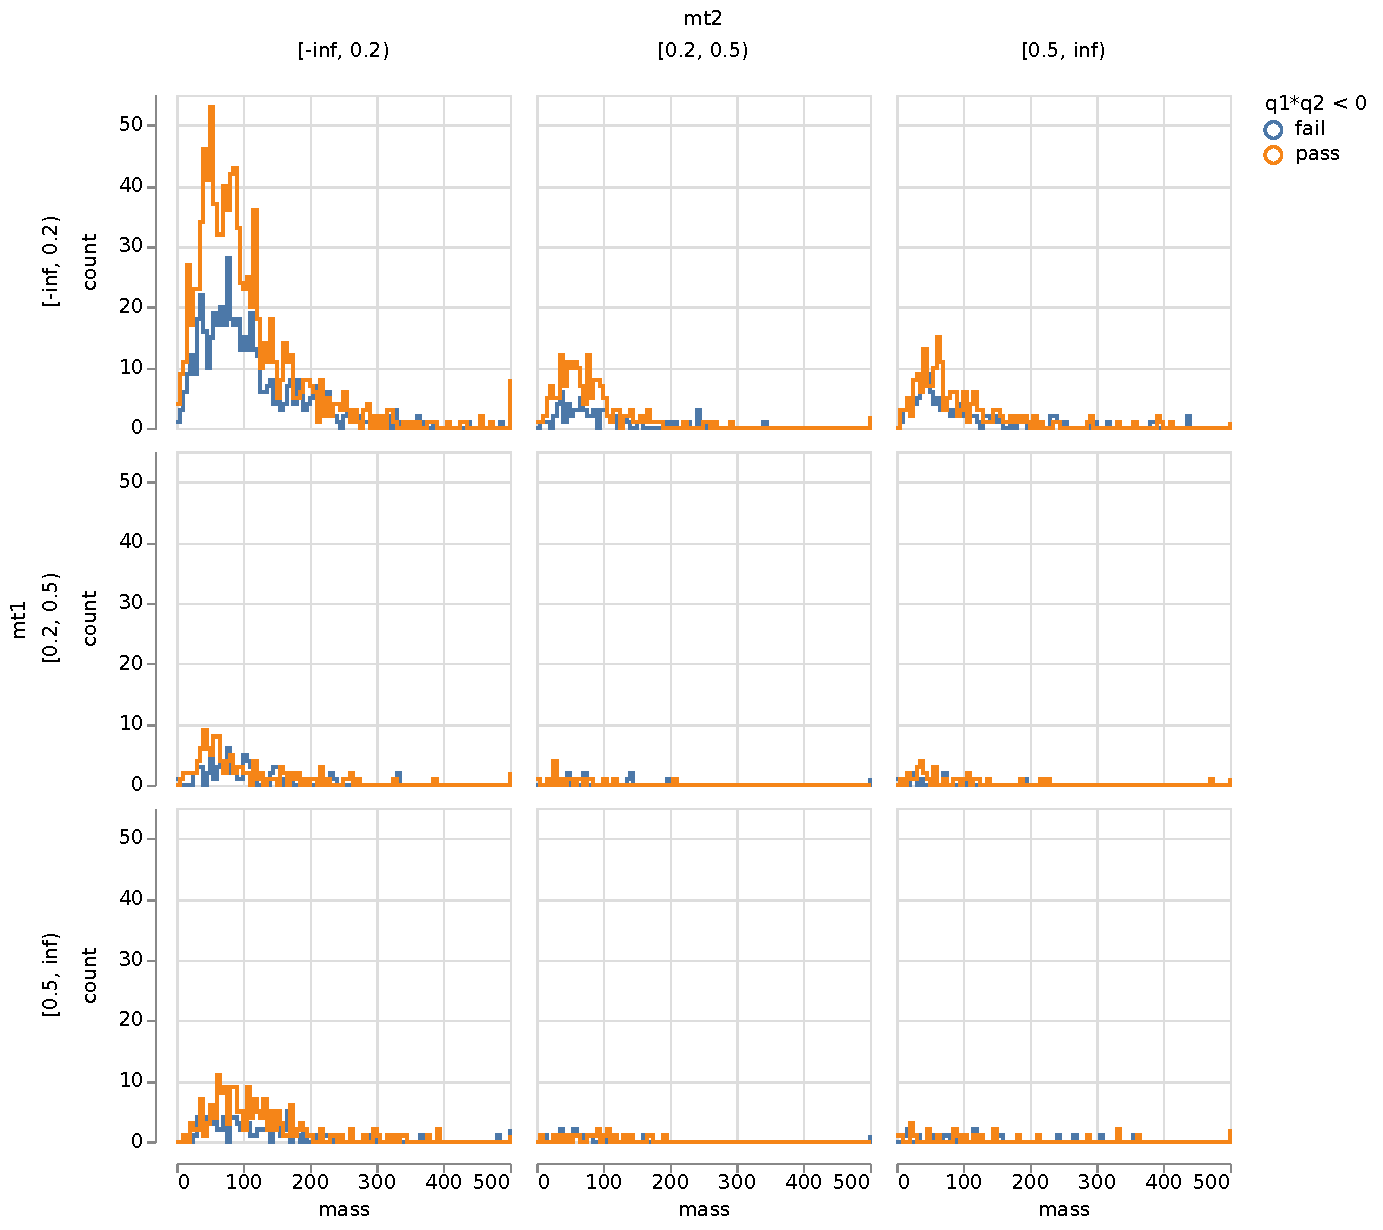
\includegraphics[height=6 cm]{pandhist_double_trellis_overlay.pdf} \hfill \mbox{ }
\end{onlyenv}
\end{frame}

\begin{frame}{From ``Pandas DataFrames for F.A.S.T.\ binned analysis at CMS''}
\begin{center}
\only<1>{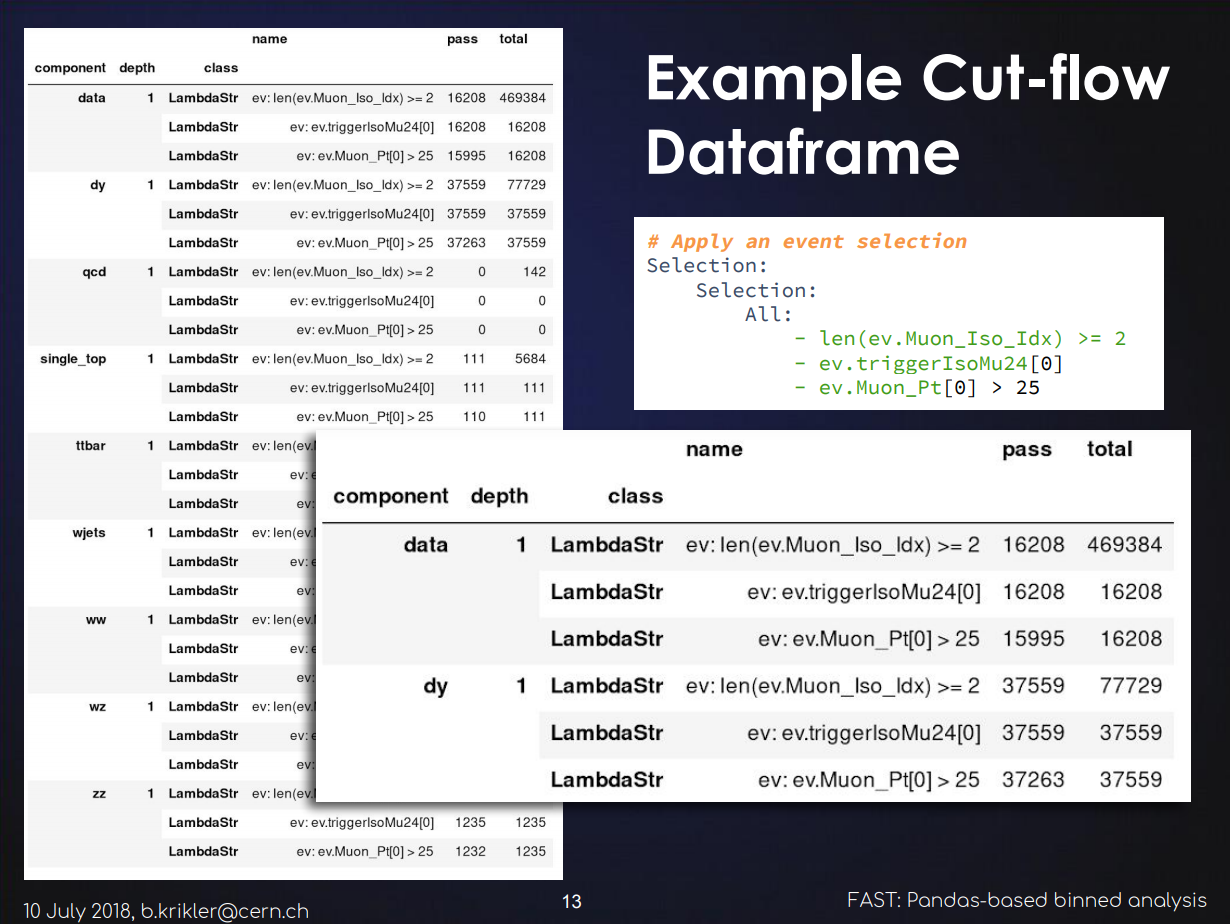
\includegraphics[width=0.75\linewidth]{fast-slide-0.png}}\only<2>{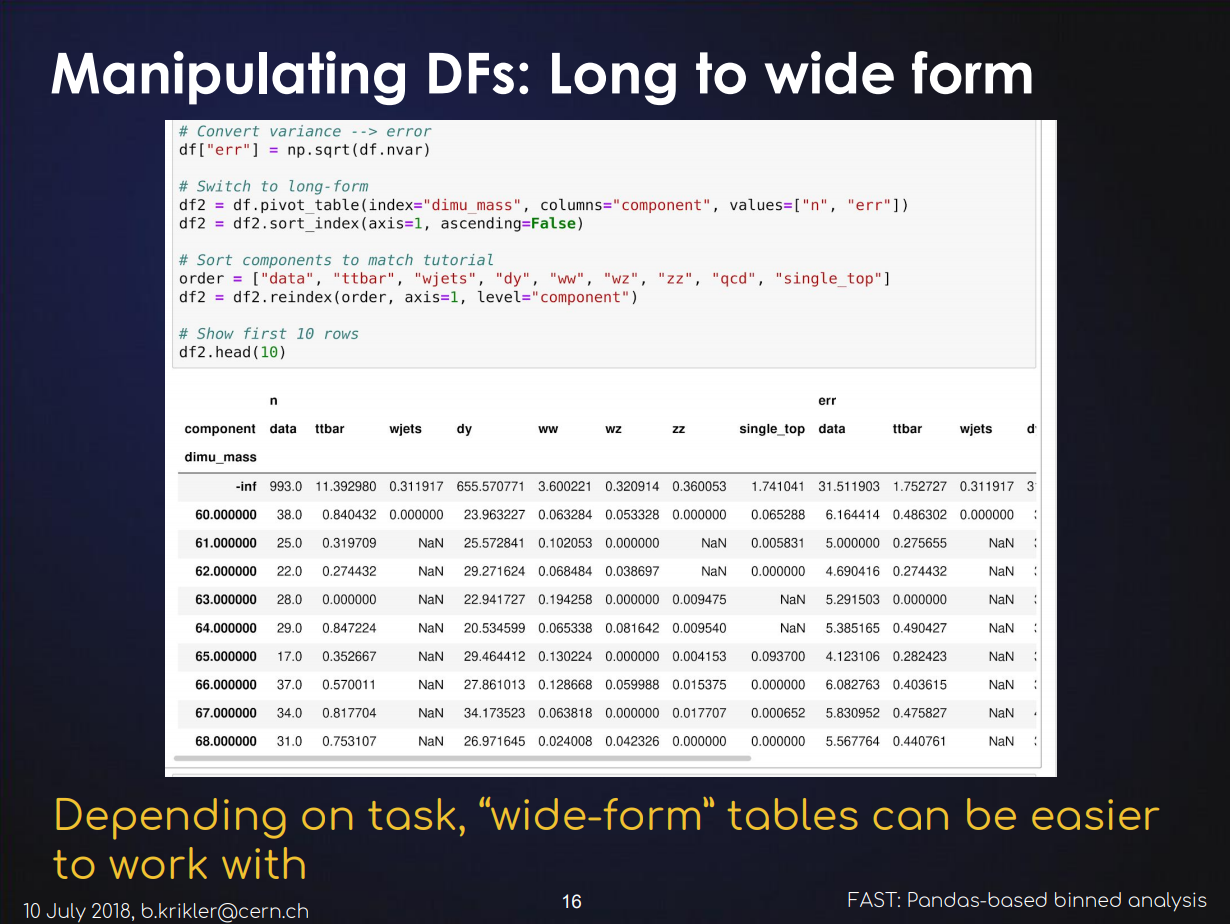
\includegraphics[width=0.75\linewidth]{fast-slide-2.png}}
\end{center}

\vspace{-8 cm}
\hfill \mbox{\begin{minipage}{2 cm}
\small Pandas DataFrames filled by \\ \textcolor{darkblue}{AlphaTwirl}, analyzed by \\ \textcolor{darkblue}{F.A.S.T.}
\end{minipage} \hspace{-0.75 cm}}
\vspace{8 cm}
\end{frame}

\begin{frame}{}
\huge
\vspace{0.5 cm}
\begin{center}
\textcolor{darkblue}{Advanced histogramming}

\large
\vspace{0.5 cm}
very physics-specific
\end{center}
\end{frame}

\begin{frame}{Advanced histogramming}
\Large
\vspace{0.25 cm}
The histograms themselves, however, are more sophisticated in particle physics software than elsewhere.

\large
\begin{itemize}\setlength{\itemsep}{0.25 cm}
\item<2-> As far as I have found, \underline{\it only} particle physics packages \textcolor{gray}{(ROOT, YODA, go-hep/hbook, AIDA, HippoDraw, Jas3, mn\_fit, PAW, HBOOK)} \\ conceive of histograms as containers to be filled.

\vspace{0.25 cm}
{\normalsize \textcolor{darkblue}{Exception:} Boost.Histogram, currently under review (Hans Dembinski, LHCb)}

\item<3-> In non-physics packages, ``histogram'' is more of a display option than an analysis tool, with no way to access contents or control binnning.

\item<4-> Profile plots are only in our tools.

\item<5-> Good log-scale handling is hard to find, too.
\end{itemize}

\begin{center}
\uncover<6->{\textcolor{red}{\Large These features are our responsibility.}}
\end{center}
\end{frame}

\begin{frame}{}
\huge
\vspace{0.5 cm}
\begin{center}
\textcolor{darkblue}{Machine learning versus ansatz fitting}
\end{center}
\end{frame}

\begin{frame}{Machine learning versus ansatz fitting}
\Large
\vspace{0.5 cm}
\textcolor{darkblue}{Machine learning:} \textcolor{darkorange}{\bf it's just fitting.}

\large
\vspace{0.5 cm}
\uncover<2->{It's fitting with thousands of free parameters, where the goal is not to find a global minimum or understand the limiting value of those parameters, but to generate, recognize, or classify patterns.}

\vspace{0.5 cm}
\uncover<3->{Ansatz fitting, however, optimizes a theory-driven function of few parameters, and the exact shape of the minimum has implications for the theory.}

\vspace{0.5 cm}
\uncover<4->{\textcolor{darkblue}{\Large Qualitatively different purposes:} \textcolor{darkorange}{\Large\bf both needed.}}

\vspace{0.5 cm}
\uncover<5->{We can look to industry for machine learning innovations, but the best ansatz fitters are in our field: RooFit, GooFit, HistFitter, HistFactory, Combiner, pyhf\ldots}
\end{frame}

\begin{frame}{Areas of overlap}
\Large
\vspace{1 cm}
\begin{columns}
\column{1.03\linewidth}
\begin{columns}[t]
\column{0.5\linewidth}
\mbox{\hspace{0.25 cm}\underline{What they've got}}

\vspace{0.25 cm}
\begin{enumerate}
\item \only<1-3>{Distributed DAG processing}\only<4>{\textcolor{darkorange}{\bf Distributed DAG processing}}
\item \only<1-2>{Indexed analysis}\only<3>{\textcolor{darkorange}{\bf Indexed analysis}}\only<4>{Indexed analysis}
\item \only<1>{Machine learning}\only<2>{\textcolor{darkorange}{\bf Machine learning}}\only<3-4>{Machine learning}
\end{enumerate}

\column{0.5\linewidth}
\mbox{\hspace{0.45 cm}\underline{What we'd need}}

\vspace{0.25 cm}
\begin{enumerate}
\item \only<1>{Nested data structures}\only<2>{\textcolor{darkorange}{\bf Nested data structures}}\only<3-4>{Nested data structures}
\item \only<1-2>{Advanced histogramming}\only<3>{\textcolor{darkorange}{\bf Advanced histogramming}}\only<4>{Advanced histogramming}
\item \only<1-3>{Ansatz fitting}\only<4>{\textcolor{darkorange}{\bf Ansatz fitting}}
\end{enumerate}
\end{columns}

\large
\vspace{1 cm}
\only<1>{\mbox{ }\vspace{3\baselineskip}}\only<2>{\textcolor{darkorange}{\bf Nearly all ML techniques require flattened or sequences of flattened data,} \\ but we have real problems that need nested data: e.g.\ classifying $N_i$ jets per event (nested, unordered sets). RNNs and LSTMs (for non-nested, ordered sequences) are designed for a different data type!}\only<3>{\textcolor{darkorange}{\bf F.A.S.T.\ and histbook are incorporating Pandas indexing into advanced histogramming.}\vspace{2\baselineskip}}\only<4>{\textcolor{darkorange}{\bf As fits get bigger, they may need to be distributed, for instance with iterative map-reduce.}\vspace{2\baselineskip}}

\mbox{ }
\end{columns}
\end{frame}

\begin{frame}{Conclusions}
\Large
\vspace{0.75 cm}
\textcolor{darkblue}{Data analysis tools outside of particle physics are mature but not a perfect fit to our needs.}

\vspace{0.35 cm}
\begin{itemize}\setlength{\itemsep}{0.35 cm}
\item Some of what we need is available now: can we use it?
\item Some exists only as physics software: can it interoperate?
\item Some of what's available is unlike anything we do now:\\an opportunity to do better physics?
\item<2-> The door swings both ways: we have things to teach the world!
\end{itemize}
\end{frame}

\end{document}
